% ====================================================================
% VİZE RAPOR ŞABLONU – Türk Masalları Derlemesi Web Sayfası
% --------------------------------------------------------------------
% DERLEME: Overleaf'te Menu > Compiler > XeLaTeX (pdfLaTeX de çalışır).
%
% KURALLAR (şablonu kullanmadan önce okuyun):
%  1. Bölüm başlıklarını SİLMEYİN ve sırasını DEĞİŞTİRMEYİN.
%  2. [KÖŞELİ PARANTEZ] içindeki ve gri renkli açıklama metinlerini
%     kendi bilgilerinizle değiştirin; açıklama metinlerini silin.
%  3. MEBİS'e YALNIZCA bu raporun PDF'ini yükleyin.
%     ZIP ve HTML dosyası YÜKLEMEYİN. Tüm kontroller GitHub'dan yapılır.
%  4. Kapaktaki GitHub ve YouTube bağlantıları doğru ve tıklanabilir
%     olmalıdır. Teslimden önce PDF'teki bağlantılara tıklayıp deneyin.
%  5. Haftalık katkı tablosundaki görseller için resim dosyalarını
%     (hafta1.png, hafta2.png, ...) Overleaf projesine yükleyin.
%     Dosya adlarında boşluk ve Türkçe karakter kullanmayın.
%     Resim yoksa tabloda "görsel ekleyin" kutusu görünür.
%  6. Yapay zekâ kullandıysanız Bölüm 5'i doldurun.
% ====================================================================
\documentclass[12pt,a4paper]{article}

\usepackage{iftex}
\ifPDFTeX
  \usepackage[T1]{fontenc}
  \usepackage[utf8]{inputenc}
\else
  \usepackage{fontspec}
\fi
\usepackage[turkish,shorthands=:!]{babel} % "=" kısayolu kapatıldı; aksi hâlde width=... ve label={} hata veriyor
\usepackage[margin=2.4cm]{geometry}
\usepackage{setspace}
\usepackage{graphicx}
\usepackage{booktabs}
\usepackage{longtable}
\usepackage{array}
\usepackage{colortbl}
\usepackage{xcolor}
\usepackage{enumitem}
\usepackage{listings}
\usepackage{amssymb}
\usepackage{caption}
\usepackage{fancyhdr}
\usepackage{hyperref}

\onehalfspacing
\setlength{\parindent}{0pt}
\setlength{\parskip}{6pt}
\setlist{itemsep=2pt, topsep=4pt}
\hypersetup{colorlinks=true, linkcolor=blue!50!black, urlcolor=blue!50!black}

\definecolor{ana}{HTML}{14325C}
\definecolor{acik}{HTML}{EEF2F8}

\lstset{basicstyle=\ttfamily\small, backgroundcolor=\color{acik},
  frame=single, rulecolor=\color{ana}, breaklines=true,
  columns=fullflexible, keepspaces=true, showstringspaces=false}

\pagestyle{fancy}
\fancyhf{}
\fancyhead[L]{\projeadi}
\fancyhead[R]{Vize Raporu}
\fancyfoot[C]{\thepage}

% ---------- Yardımcı komutlar ----------
% Haftalık tablo görseli: dosya yoksa "görsel ekleyin" kutusu çıkar
\newcommand{\haftagorsel}[1]{%
  \IfFileExists{#1}{%
    \raisebox{-\height}{\includegraphics[width=\linewidth,height=4.2cm,keepaspectratio]{#1}}%
  }{%
    \fbox{\parbox[c][2.6cm][c]{\dimexpr\linewidth-2\fboxsep-2\fboxrule\relax}{%
      \centering\small\color{gray} Ekran görüntüsü / görsel ekleyin\\ \texttt{#1}}}%
  }%
}
% Haftalık katılım kutuları.
% 1. parametre: "Ders içinde katılım sergiledim", 2. parametre: "Telafi yaptım".
% İşaretli için \boxtimes, boş için \square yazın.
\newcommand{\katilimkutulari}[2]{\par\vspace{3pt}\small $#1$ Ders içinde katılım sergiledim\par $#2$ Telafi yaptım}

% Ek görsel: dosya yoksa hiçbir şey göstermez
\newcommand{\haftaek}[1]{%
  % Not: hücre içinde \\ satırı bitirdiği için \par kullanıldı
  \IfFileExists{#1}{\par\vspace{4pt}\includegraphics[width=\linewidth,height=4.2cm,keepaspectratio]{#1}}{}%
}

% ---------- Kapak bilgileri ----------
\newcommand{\universite}{İstanbul Medipol Üniversitesi / Görsel İletişim Tasarımı}
\newcommand{\dersadi}{Programlamaya Giriş}
\newcommand{\hocaadi}{Meral Şentürk}
\newcommand{\ogrenciadi}{Berkant Özkuş}
\newcommand{\ogrencino}{86230030}
\newcommand{\projeadi}{Gizemli Masal Atlası}
% Bağlantıları tam adres olarak yazın (https:// ile başlayarak)
\newcommand{\githublink}{\url{https://github.com/berkanthrli/gizemli-masal-atlasi}}
% !!! VİDEOYU YÜKLEDİKTEN SONRA AŞAĞIDAKİ ADRESİ KENDİ VİDEO BAĞLANTINLA DEĞİŞTİR !!!
\newcommand{\youtubelink}{\url{https://www.youtube.com/watch?v=ugbjlfLZfmA}}
\newcommand{\videosuresi}{13:25}   % örnek: 14:32
\newcommand{\videogorunurluk}{Listelenmemiş}

\begin{document}

% ====================================================================
% KAPAK
% ====================================================================
\begin{titlepage}
\centering
\vspace*{1cm}
{\large \universite \par}
\vspace{1.8cm}
{\Huge\bfseries\color{ana} \projeadi \par}
\vspace{0.4cm}
{\Large Türk Masalları Derlemesi Web Sayfası \par}
{\large Vize Raporu \par}
\vspace{1.8cm}
{\large \textbf{Ders:} \dersadi \par}
{\large \textbf{Öğretim Üyesi:} \hocaadi \par}
\vspace{1.2cm}
{\large \textbf{Hazırlayan:} \ogrenciadi \par}
{\large \textbf{Öğrenci No:} \ogrencino \par}
\vspace{1.8cm}
\fbox{\parbox{0.88\linewidth}{\centering\vspace{6pt}
{\large\bfseries Proje Bağlantıları}\\[8pt]
\textbf{GitHub deposu:}\\ \githublink \\[8pt]
\textbf{YouTube sunum videosu:}\\ \youtubelink
\vspace{6pt}}}
\vfill
{\large \today \par}
\end{titlepage}

\tableofcontents
\newpage

% ====================================================================
\section{Giriş}
% ====================================================================
Bu projede Türk halk anlatı geleneğinden seçtiğim on masalı, gece ormanı ve masal kitabı
temasıyla tasarladığım tek sayfalık bir web sitesinde bir araya getirdim. Amacım, masalları
yalnızca alt alta dizmek değil, okuyucunun istediği masalı hızlıca bulabileceği ve kitap
sayfası çevirir gibi okuyabileceği bir arayüz hazırlamaktı. Sayfa \texttt{index.html} adlı tek
bir dosyadan oluşuyor; bütün stiller \texttt{<style>}, bütün betikler \texttt{<script>} etiketleri
içinde yazılı. Harici yazı tipi, kütüphane ya da görsel dosyası kullanmadığım için sayfa
internet bağlantısı olmadan da açılıp çalışıyor. Masalları kaynaktan kopyalamadım; olay örgüsünü koruyarak sade bir dille yeniden anlattım. JavaScript sayfada masal arama, türe göre
süzme, yazı boyutu ayarlama ve masalı sayfalara bölerek kitap görünümünde okutma işlerini
yapıyor. Bu raporda masalları nasıl seçtiğimi, tasarım kararlarımı, kodun mantığını, yapay
zekâ kullanımımı, haftalık ders çalışmalarımı ve test sonuçlarımı anlatıyorum.

\subsection{Proje Özeti}
\textbf{Gizemli Masal Atlası}, on Türk masalını bir ``masal rafı'' düzeninde sunan, tek
HTML dosyasından oluşan bir web sayfasıdır. Ana sayfada kullanıcı masal adına göre arama
yapabilir, masalları ``Hayvan karakterleri'', ``Büyü ve gizem'' ve ``İnsan hikâyeleri''
türlerine göre süzebilir ve metin boyutunu büyütebilir. Bir masalın ``Masalı oku'' düğmesine
basıldığında sayfa değişmeden bir kitap penceresi açılır: önce masalın adının yazdığı kapak
görünür, ``Kitabı aç'' ile metin sayfalara bölünür ve ``Önceki / Sonraki'' düğmeleri ya da
klavyedeki ok tuşlarıyla okunur. Masalların tam metinleri ayrıca ``Masal arşivi''
bölümünde, derleyen bilgileriyle birlikte yer alır.

\subsection{Gereksinimlerin Karşılanması}
\begin{center}
\rowcolors{2}{acik}{white}
\begin{tabular}{@{}p{8.2cm}c@{}}
\toprule
\rowcolor{ana}\textcolor{white}{\textbf{Gereksinim}} & \textcolor{white}{\textbf{Durum}} \\
\midrule
Masal sayısı 8--12 arasında (10 masal)              & $\boxtimes$ \\
Tek HTML dosyası (\texttt{index.html})              & $\boxtimes$ \\
Stil kodları içsel (\texttt{<style>} içinde)        & $\boxtimes$ \\
Betik kodları içsel (\texttt{<script>} içinde)      & $\boxtimes$ \\
İnternetsiz açılıp çalışıyor                        & $\boxtimes$ \\
JavaScript sayfada anlamlı bir işlev görüyor        & $\boxtimes$ \\
Masal metinleri kendi cümlelerimle yazıldı          & $\boxtimes$ \\
Sayfa telefonda da düzgün görünüyor                 & $\boxtimes$ \\
\bottomrule
\end{tabular}
\end{center}
Masalların aslı Türk Masal Külliyatı projesinin \texttt{masal.gov.tr} arşivindedir. Metinleri
oradan kopyalamak yerine olayları, karakterleri ve masalın verdiği öğüdü koruyarak cümleleri
baştan kurdum, uzun betimlemeleri kısaltıp çocukların rahat okuyacağı bir dil kullandım. Bu
yeniden anlatımda yapay zekâdan yardım aldım (bkz.\ Bölüm 5); çıkan metinleri tek tek okuyup
kaynak masalla karşılaştırdım. Her masalın sonunda kaynak ve derleyenin adı yazılıdır.

% ====================================================================
\section{Masalların Seçimi}
% ====================================================================
Masalları seçerken üç ölçüt kullandım: (1) sayfadaki süzgeç türlerinin her birinde en az
iki masal olması (hayvan, büyü-gizem, insan hikâyesi), (2) masalların farklı değerleri
işlemesi (yardımlaşma, sevgi, zekâ, bencillikten uzak durma) ve (3) metnin bir oturuşta,
kitap görünümünde birkaç sayfada okunabilecek uzunlukta olması. Bütün masallar Türk Masal
Külliyatı arşivindeki (\texttt{masal.gov.tr}) derlemelerden seçilmiş ve yeniden anlatılmıştır.

\begin{longtable}{@{}c>{\raggedright\arraybackslash}p{4cm}>{\raggedright\arraybackslash}p{3cm}>{\raggedright\arraybackslash}p{5.4cm}@{}}
\toprule
\textbf{No} & \textbf{Masal} & \textbf{Tür} & \textbf{Seçilme nedeni} \\
\midrule
\endhead
1 & Altın Saçlı Kız & Büyü ve gizem & Atlasın en uzun ve en ``masalsı'' anlatısı; iyilik ve güvenin zamanla kazanılması temasını işliyor. \\
2 & Altın Top & İnsan hikâyesi & Zengin ve yoksul komşu karşılaştırmasıyla mutluluğun yalnızca paraya bağlı olmadığını anlatıyor. \\
3 & Tütüncü Kızı & İnsan hikâyesi & Zekâsıyla öne çıkan bir kız kahramanı var; kısa ve akıcı olduğu için okuyucuya iyi bir başlangıç. \\
4 & Tombul Gözleme & Hayvan karakterleri & Tekrarlı yapısı ve konuşan hayvanlarıyla çocuklara yönelik, eğlenceli bir zincir masal. \\
5 & Sevgiyle Akan Gözyaşları & Büyü ve gizem & Padişah kızı ile çobanın sevgisini anlatıyor; klasik tekerlemeyle açılan geleneksel kurguya örnek. \\
6 & Sihirli Tencere & Büyü ve gizem & Olağanüstü bir nesnenin (sihirli tencere) olayları değiştirdiği, üç kardeş motifli bir masal. \\
7 & Perili Ev & Büyü ve gizem & Atlasın ``gizemli'' temasına en uygun masal; bencillik yerine dayanışmanın kazandığını anlatıyor. \\
8 & Kocakarıyla Tilki & Hayvan karakterleri & Tilkinin kuyruğunu geri almak için zincirleme iyilikler istediği, tekrar yapısıyla tanınan bir zincir masal. \\
9 & Aslan Padişah ile Fare & Hayvan karakterleri & ``Kimseyi küçük görme'' öğüdünü güçlü ve küçük iki hayvanın dostluğuyla veriyor. \\
10 & Tilki ile Aslan & Hayvan karakterleri & Kurnaz tilki karakterinin mizahi bir örneği; kısa olduğu için sayfa çevirme özelliğini denemeye uygun. \\
\bottomrule
\end{longtable}

% ====================================================================
\section{Tasarım Kararları}
% ====================================================================
Sayfanın tasarımını kendim belirledim; hazır web sitesi şablonu ya da tema paketi
kullanmadım. Tasarımda temel fikir, ``masallar gece anlatılır'' düşüncesinden yola çıkarak
okuyucuyu ay ışıklı bir gece ormanından bir masal kütüphanesine götürmekti.

\subsection{Konuya Uygunluk}
Türk masalları geleneksel olarak akşamları, ninelerin anlattığı hikâyelerdir; bu yüzden
giriş bölümünü koyu lacivert bir gece göğü, ay ve yıldızlarla kurdum. Ay ve dağ silüetleri
dışarıdan görsel dosyası olarak değil, CSS gradyanları ve satır içi bir SVG ile çizildi;
böylece sayfa hem tek dosya kalıyor hem de internetsiz çalışıyor. Altın sarısı vurgular
masallardaki ``altın top'', ``altın saç'' gibi motifleri ve eski kitap yaldızlarını
çağrıştırıyor. Masal kartları ve okuma alanı ise eski bir masal kitabının sayfalarını
hatırlatan parşömen renginde. Masalın kitap gibi açılması da ``masal kitabı okuma''
deneyimini ekrana taşımak için seçtiğim bir karar.

\subsection{Renk Paleti ve Yazı Tipi}
\begin{center}
\rowcolors{2}{acik}{white}
\begin{tabular}{@{}llp{6.4cm}@{}}
\toprule
\rowcolor{ana}\textcolor{white}{\textbf{Ad}} & \textcolor{white}{\textbf{Kod}} & \textcolor{white}{\textbf{Nerede / neden kullandınız?}} \\
\midrule
Gece laciverti & \texttt{\#09152F} & Üst menü, giriş bölümü ve kitap kapağı. Gece masalı havasını veriyor. \\
Altın sarısı & \texttt{\#E9C979} & Düğmeler, menü çizgisi, vurgular. Lacivert zemin üzerinde 11,3:1 karşıtlık sağlıyor. \\
Parşömen & \texttt{\#F8EFD9} & Masal kartları ve okuma sayfaları; eski kitap kâğıdını çağrıştırıyor, beyaza göre gözü daha az yoruyor. \\
Mürekkep & \texttt{\#222B42} & Gövde metinleri. Parşömen üzerinde 12,3:1 karşıtlık, yani rahat okunuyor. \\
Arial Rounded MT Bold / Trebuchet MS & -- & Sistem yazı tipleri. Yuvarlak hatlı başlık yazısı çocuk kitaplarını andırıyor; Trebuchet MS ekranda okunaklı. İnternetsiz çalışması için harici yazı tipi yüklemedim. \\
\bottomrule
\end{tabular}
\end{center}

\subsection{Okunabilirlik, Gezinme ve Duyarlı Tasarım}
\begin{itemize}
  \item \textbf{Okunabilirlik:} Masal metni yaklaşık 17 piksel (1,06--1,08\,rem) boyutunda ve
  1,95 satır aralığıyla yazılıyor. İçerik en fazla 1200 piksel genişliğinde bir alana
  sığdırıldı, kenarlarda boşluk bırakıldı. Metin--zemin karşıtlık oranı 11:1'in üzerinde.
  Kullanıcı isterse ``Yazı boyutu'' menüsünden metni \%10 ya da \%20 büyütebiliyor.
  \item \textbf{Gezinme:} Üstteki sabit menü ``Masallar'', ``Masal arşivi'' ve ``Hakkında''
  bölümlerine götürüyor. Masal rafında arama kutusu ve tür süzgeci var; aranan masal yoksa
  ``Bu aramayla eşleşen masal bulunamadı'' uyarısı çıkıyor. Her masal tek tıklamayla kitap
  penceresinde açılıyor, arşivdeki masalların altında ``Başa dön'' düğmesi bulunuyor.
  \item \textbf{Duyarlı tasarım:} Masal kartları bilgisayarda 3 sütun, 850 pikselin altında
  2 sütun, 560 pikselin altında tek sütun oluyor. Telefonda menü alt alta diziliyor, kitap
  penceresinin yüksekliği ve yazı boyutu ekrana göre küçülüyor.
  \item \textbf{Tutarlılık:} Renkler \texttt{:root} içinde değişken olarak tanımlandı ve her
  yerde bu değişkenler kullanıldı. Her bölüm aynı yapıda (küçük altın üst başlık, büyük
  başlık, açıklama) başlıyor; kartlar ve düğmeler aynı köşe yuvarlaklığını taşıyor.
\end{itemize}

\subsection{Ekran Görüntüleri}
\begin{figure}[h]
  \centering
  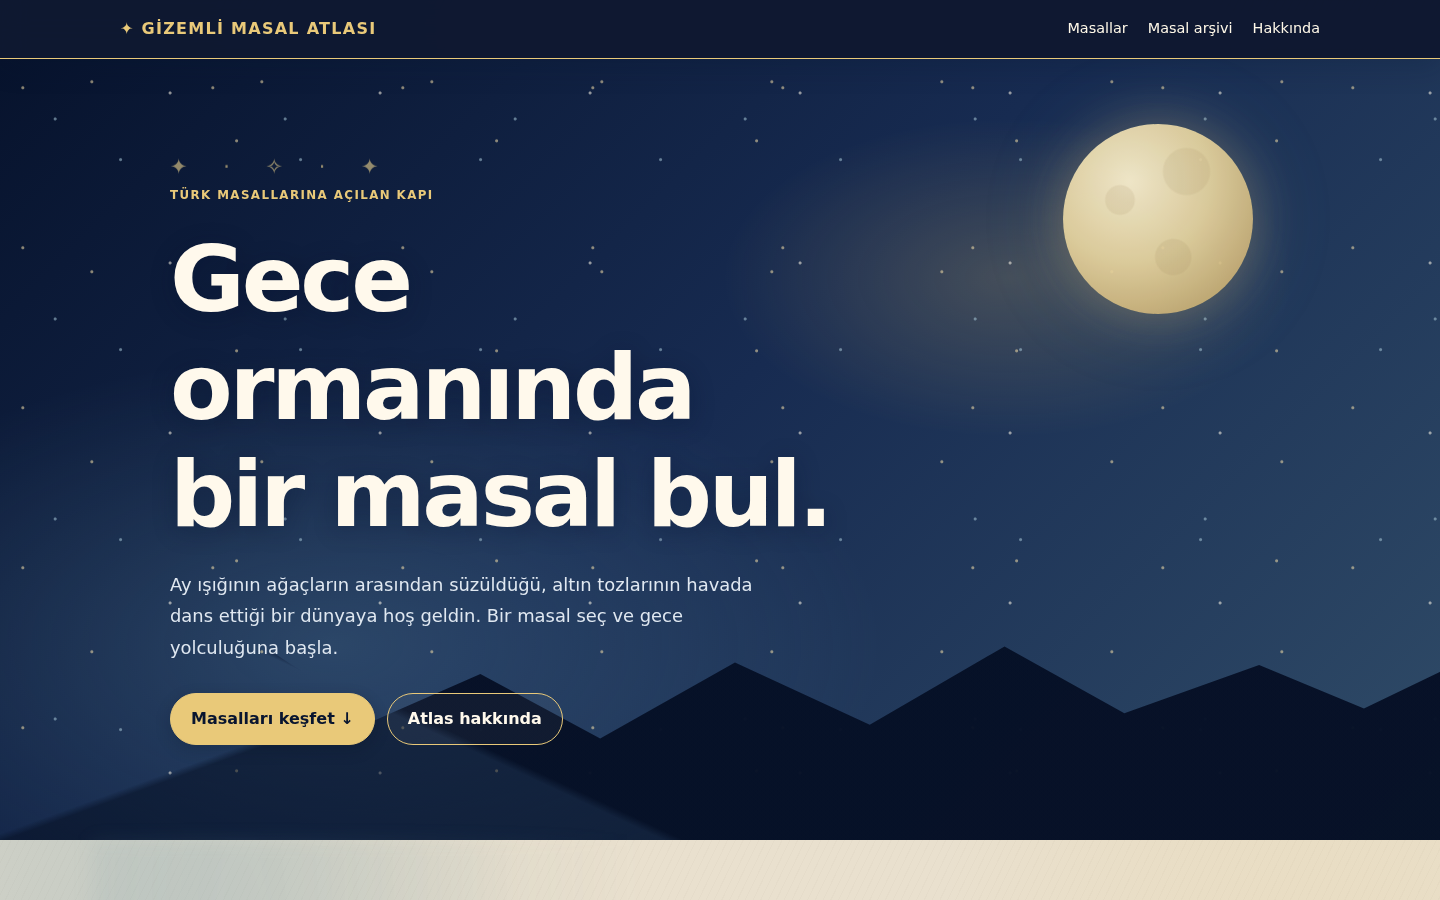
\includegraphics[width=0.9\textwidth]{ekran-masaustu.png}
  \caption{Sayfanın bilgisayar görünümü: giriş bölümü}
\end{figure}
\begin{figure}[h]
  \centering
  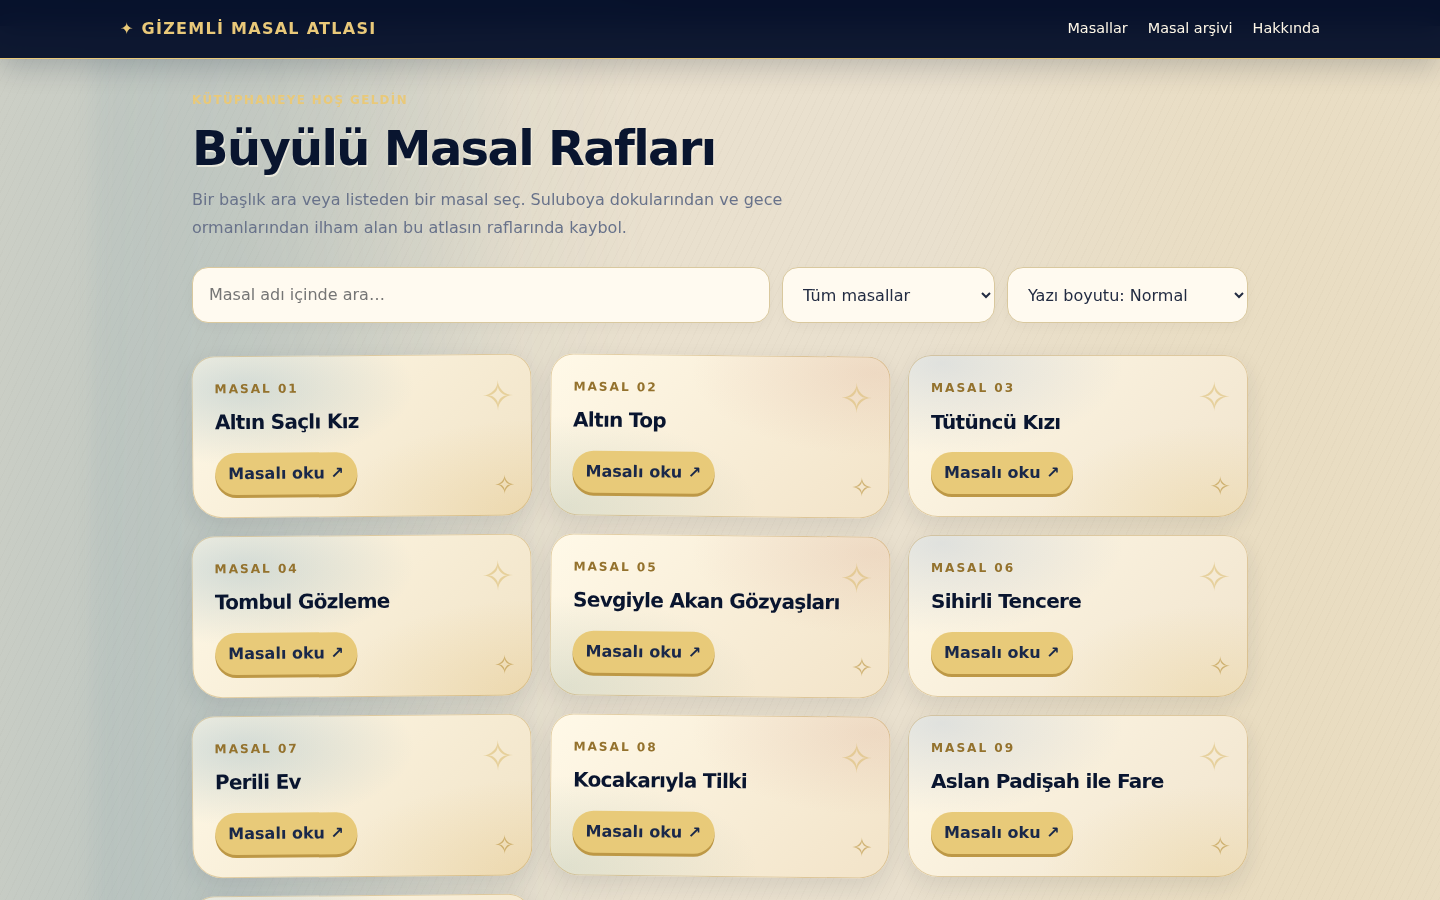
\includegraphics[width=0.9\textwidth]{ekran-masaustu-liste.png}
  \caption{Masal rafı: arama kutusu, tür süzgeci, yazı boyutu ve masal kartları}
\end{figure}
\begin{figure}[h]
  \centering
  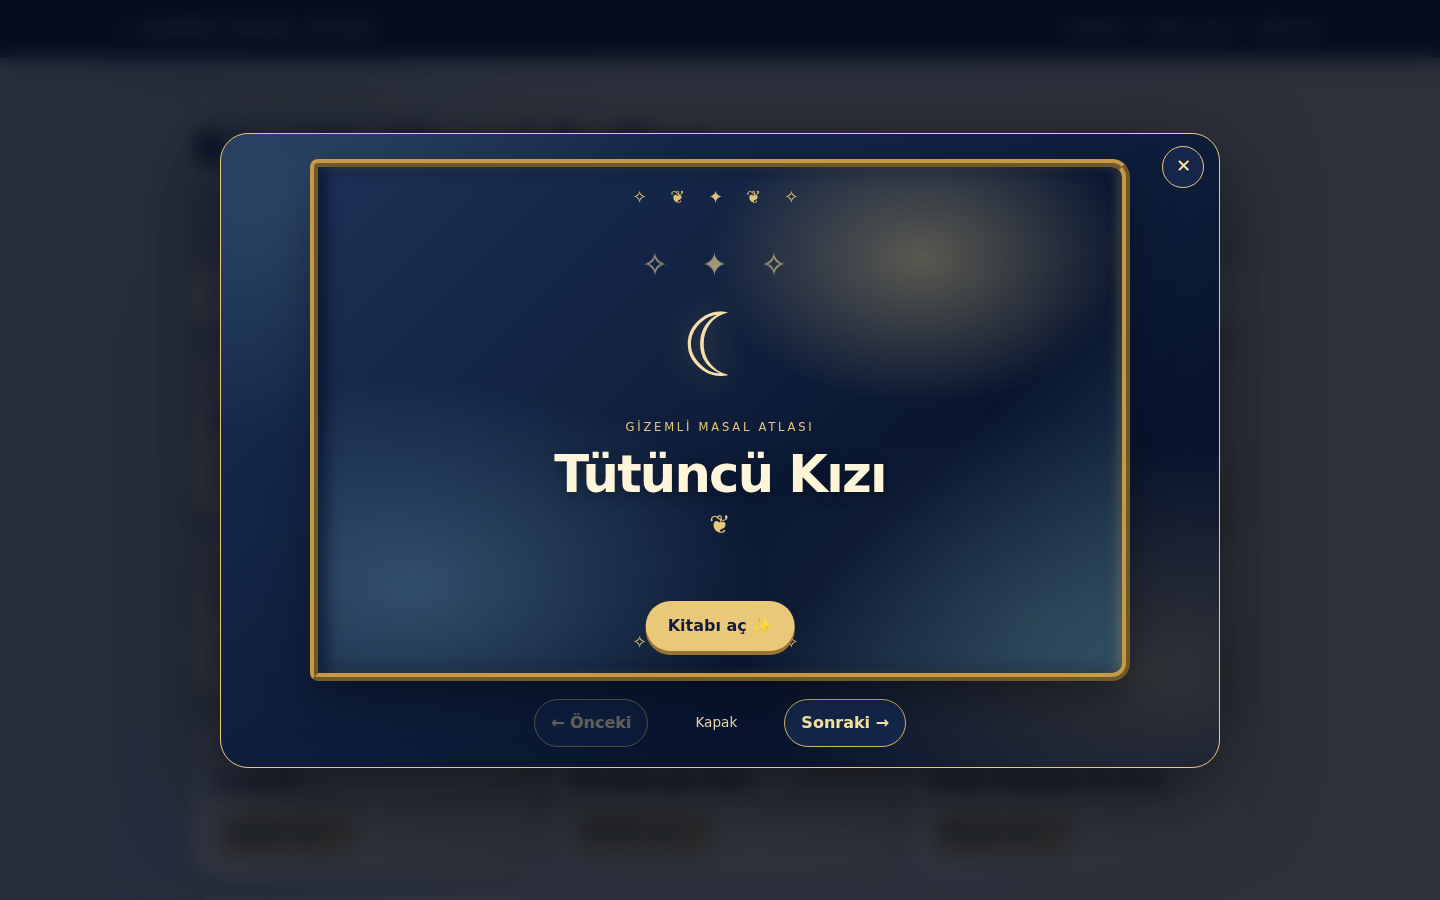
\includegraphics[width=0.48\textwidth]{ekran-kitap-kapak.png}\hfill
  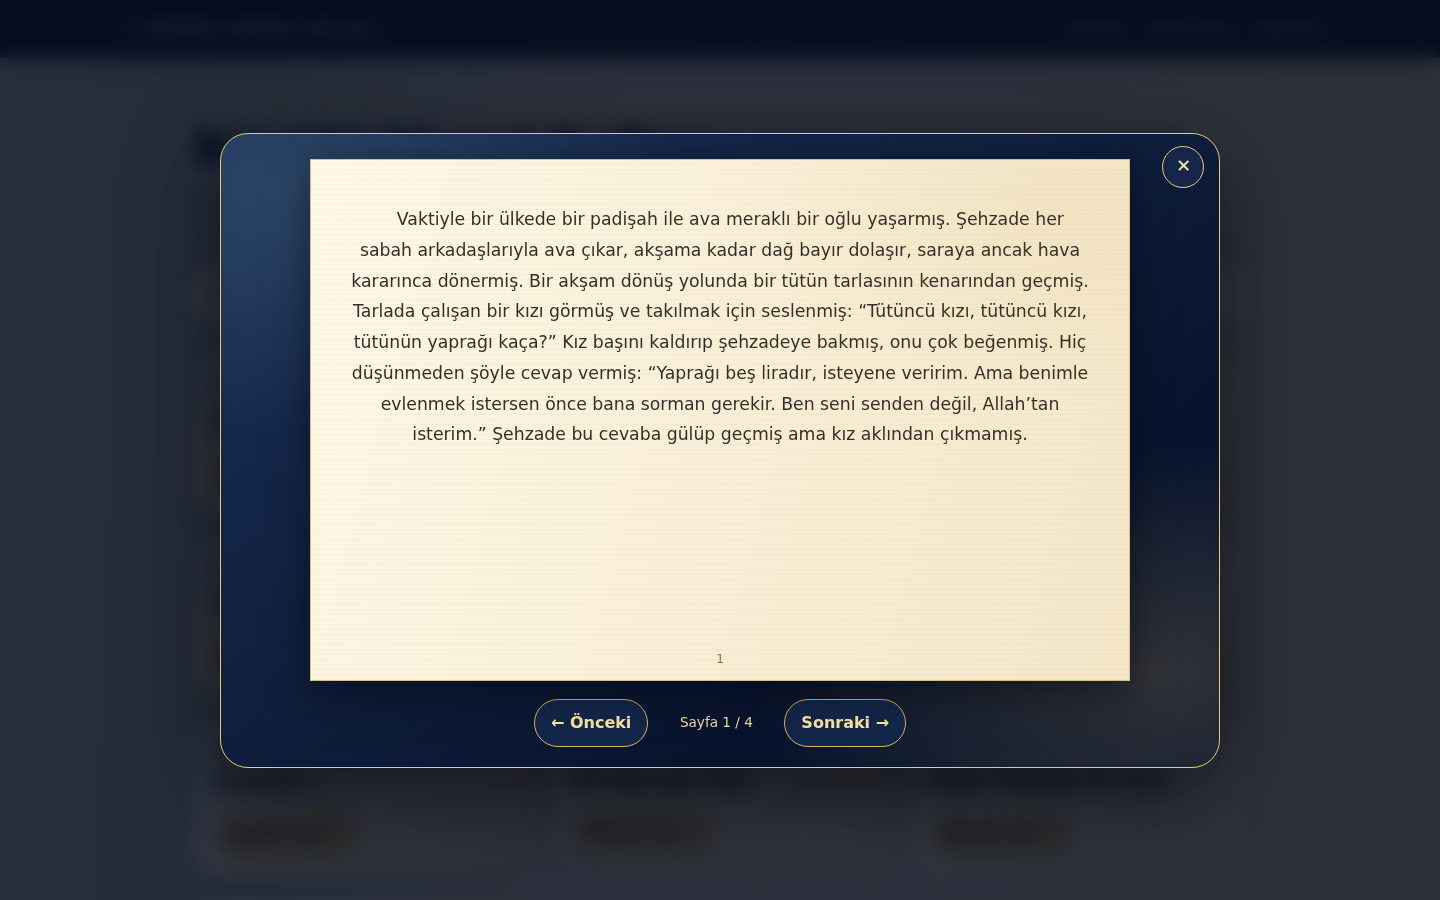
\includegraphics[width=0.48\textwidth]{ekran-kitap-sayfa.png}
  \caption{Kitap penceresi: kapak (solda) ve masal sayfası (sağda)}
\end{figure}
\begin{figure}[h]
  \centering
  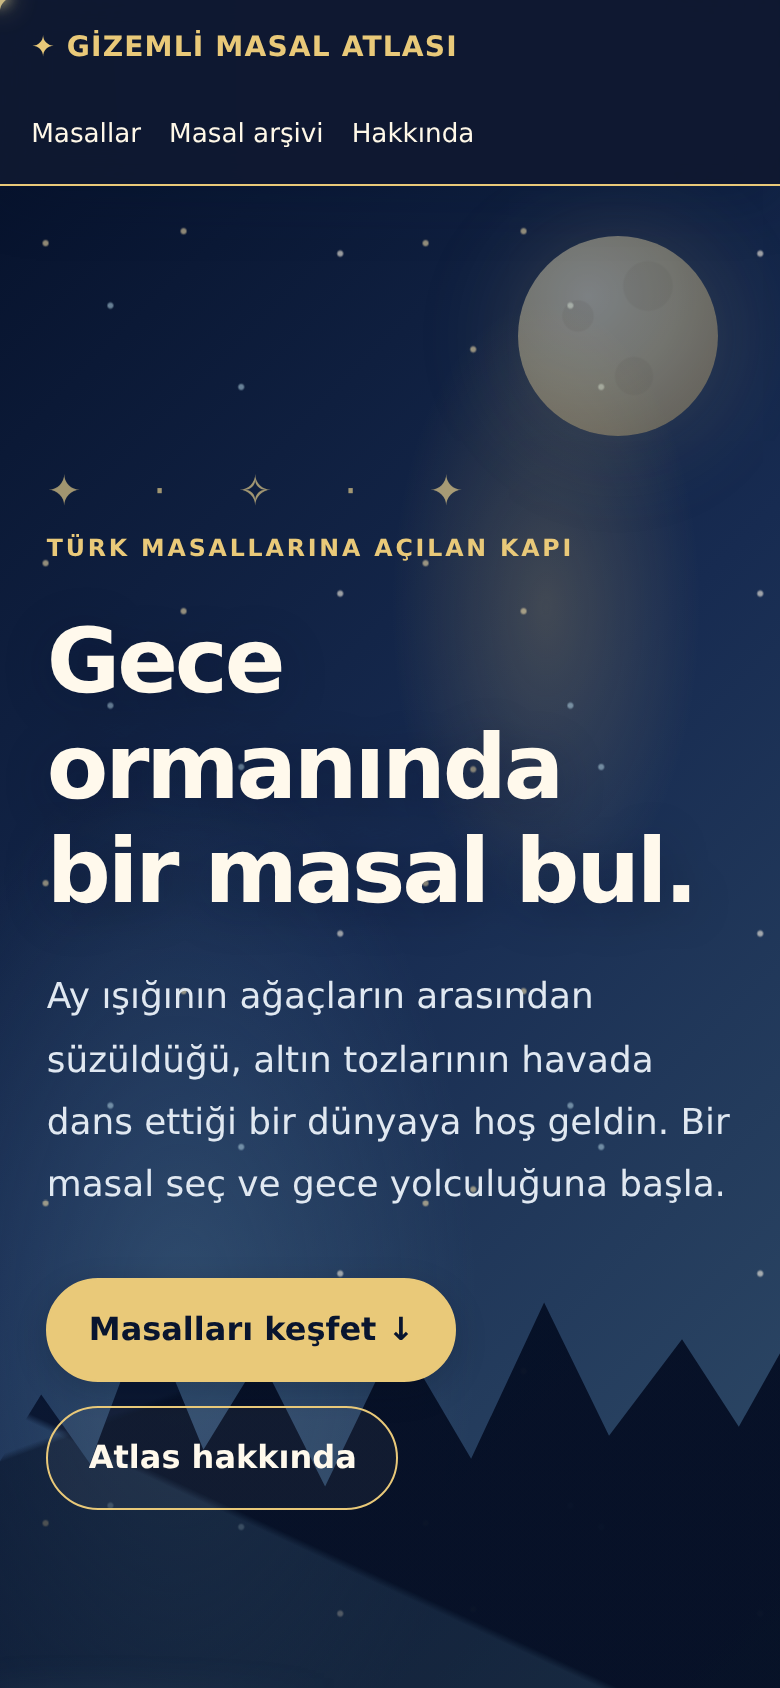
\includegraphics[width=0.28\textwidth]{ekran-mobil.png}\hspace{0.03\textwidth}
  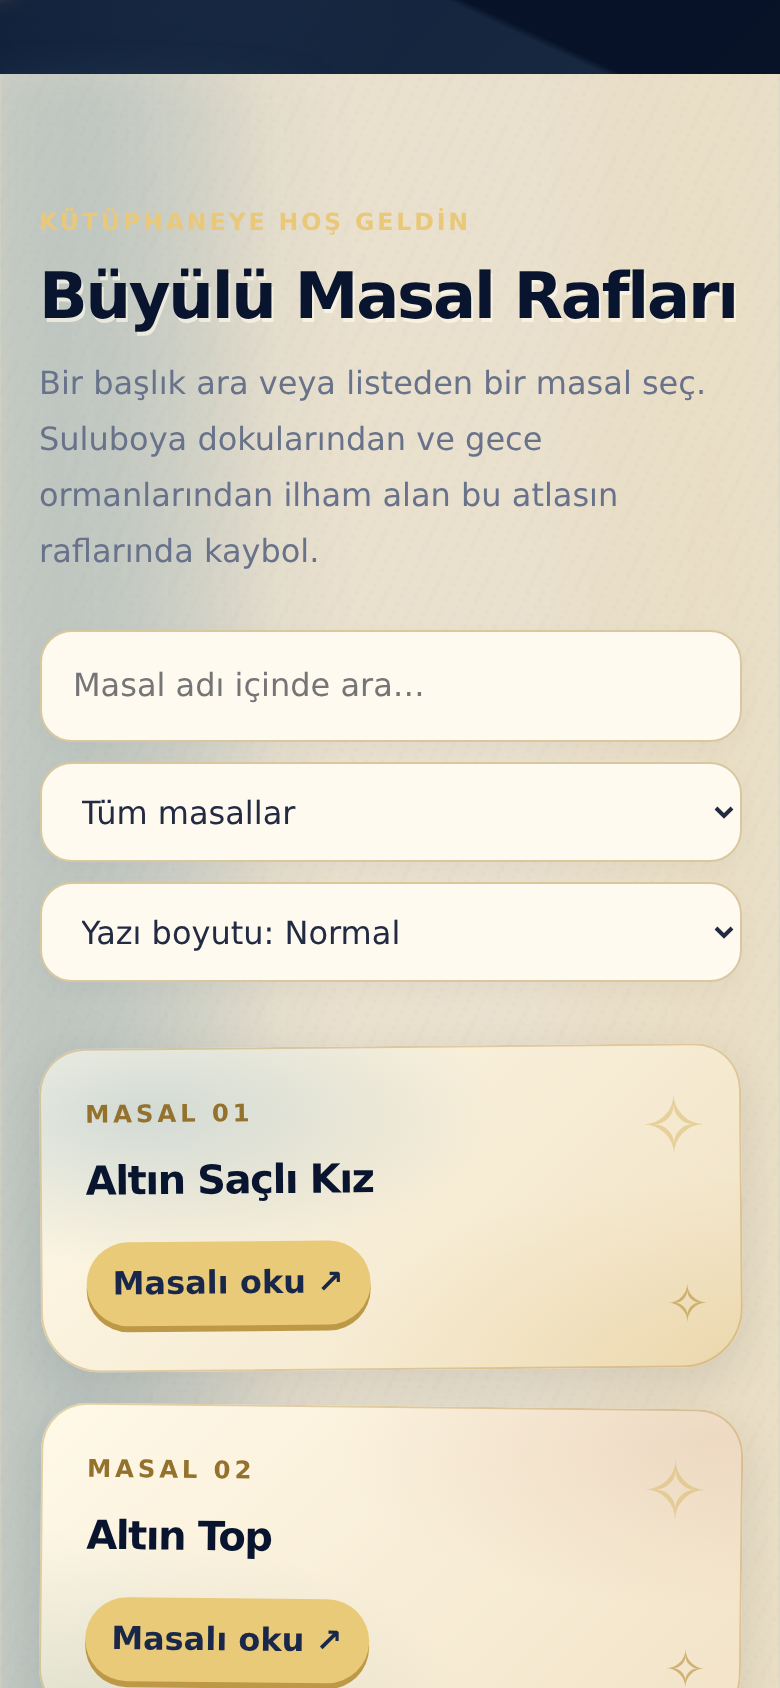
\includegraphics[width=0.28\textwidth]{ekran-mobil-liste.png}\hspace{0.03\textwidth}
  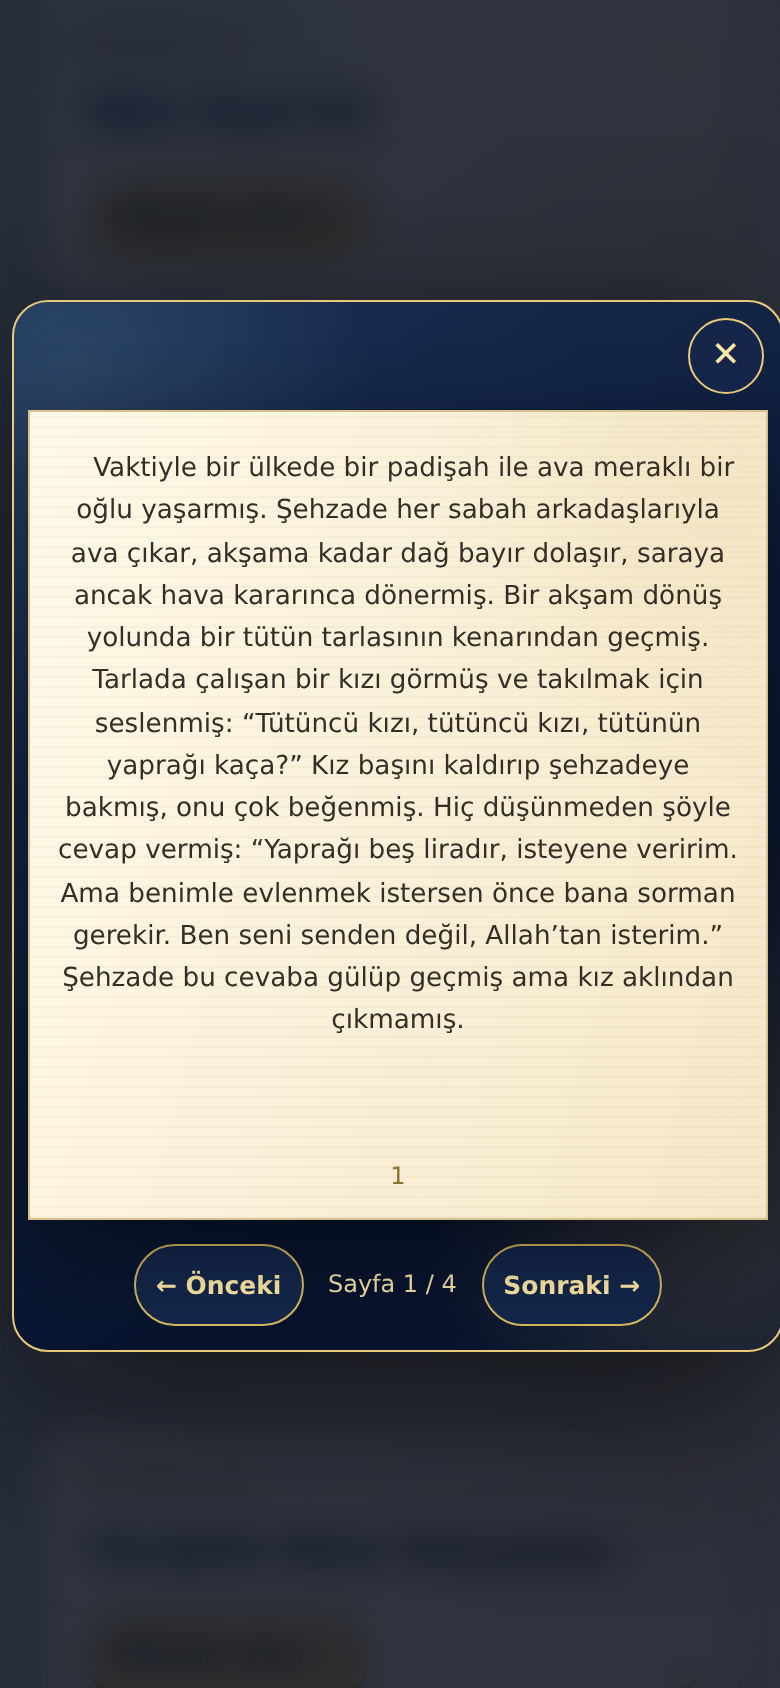
\includegraphics[width=0.28\textwidth]{ekran-mobil-kitap.png}
  \caption{Sayfanın telefon görünümü (390 piksel genişlik): giriş, tek sütunlu masal rafı ve kitap penceresi}
\end{figure}
\clearpage

% ====================================================================
\section{Gerçekleştirme}
% ====================================================================
\subsection{HTML Yapısı}
Sayfa yukarıdan aşağıya şu bölümlerden oluşuyor: \texttt{<header>} içinde \texttt{<nav>} ile
sabit üst menü; giriş (hero) \texttt{<section>}'ı; \texttt{<main>} içinde masal rafı
(\texttt{\#masallar}), masal arşivi (\texttt{\#arsiv}) ve hakkında (\texttt{\#hakkinda})
bölümleri; açılır kitap penceresi (\texttt{\#bookOverlay}) ve \texttt{<footer>}. Masal rafındaki
her masal bir \texttt{<article class="index-card">}; bu etiket \texttt{data-title} (aramada
kullanılan küçük harfli ad) ve \texttt{data-category} (süzgeçte kullanılan tür) özniteliklerini
taşıyor. Arama için \texttt{<input type="search">}, süzgeç ve yazı boyutu için iki
\texttt{<select>} kullandım. Kitap penceresi \texttt{role="dialog"} ve \texttt{aria-modal}
ile işaretlendi; dekoratif öğelere \texttt{aria-hidden="true"} verildi.

\subsection{İçsel CSS}
Bütün renkler \texttt{:root} içinde CSS değişkeni olarak tanımlı, böylece bir rengi tek
yerden değiştirebiliyorum. Masal kartlarının düzeni CSS Grid ile, araç çubuğu ve menü
Flexbox ile yapıldı. Duyarlı tasarım için \texttt{@media} sorgularıyla sütun sayısı
düşürülüyor; \texttt{clamp()} ile yazı boyutu ve kitap yüksekliği ekrana göre esniyor.
Hareket azaltmayı seçen kullanıcılar için \texttt{prefers-reduced-motion} ile animasyonlar
kapatılıyor, yazdırmada da menü ve düğmeler gizleniyor.

\begin{lstlisting}[caption={İçsel CSS'ten önemli bir bölüm}]
:root{
 --night:#09152f; --gold:#e9c979;
 --parchment:#f8efd9; --ink:#222b42;
}
.story-index{display:grid;
 grid-template-columns:repeat(3,minmax(0,1fr)); gap:18px}
/* tablet: 2 sutun */
@media(max-width:850px){
 .story-index{grid-template-columns:repeat(2,minmax(0,1fr))}}
/* telefon: tek sutun */
@media(max-width:560px){
 .story-index{grid-template-columns:1fr}}
\end{lstlisting}

\subsection{İçsel JavaScript}
Masal metinleri HTML içinde, arşivdeki \texttt{<article class="story-card">} öğelerinde
duruyor; JavaScript bu öğeleri \texttt{querySelectorAll} ile diziye alıp kullanıyor.
Önemli fonksiyonlar şunlar:
\begin{itemize}
  \item \texttt{filterStories()}: Arama kutusundaki yazıyı Türkçe kurallarına göre küçük
  harfe çeviriyor (\texttt{toLocaleLowerCase('tr-TR')}), her kartın adı ve türüyle
  karşılaştırıp uymayanları gizliyor, hiç sonuç yoksa uyarıyı gösteriyor.
  Arama kutusunun \texttt{input}, süzgecin \texttt{change} olayına bağlı.
  \item \texttt{chunks(text)}: Masal metnini yaklaşık 650 karakterlik parçalara bölüyor;
  parçayı mümkünse cümle sonunda (nokta, ünlem, soru işareti), olmazsa bir boşlukta kesiyor.
  Her parça kitapta bir sayfa oluyor.
  \item \texttt{openBook(id)}, \texttt{begin()}, \texttt{turn(dir)}, \texttt{close()}: Kitabı
  kapakla açıyor, sayfaları oluşturuyor, ileri-geri çeviriyor (ilk sayfada ``Önceki'' kapağa
  dönüyor) ve pencereyi kapatıyor. Sayfa durumu ``Sayfa 2 / 5'' gibi gösteriliyor.
\end{itemize}
Olaylar \texttt{addEventListener} ile bağlandı. ``Masalı oku'' bağlantılarına tıklama
belge düzeyinde yakalanıyor ve \texttt{preventDefault()} ile sayfanın başka adrese gitmesi
engelleniyor. Klavyede \texttt{Escape} pencereyi kapatıyor, sol/sağ ok tuşları sayfa
çeviriyor. Metni sayfaya eklerken \texttt{esc()} fonksiyonu özel karakterleri
dönüştürüyor, böylece metin HTML olarak yorumlanmıyor.

\begin{lstlisting}[caption={İçsel JavaScript'ten önemli bir bölüm}]
function filterStories(){
  const query=searchInput.value.trim().toLocaleLowerCase('tr-TR');
  const category=categorySelect.value;
  let visible=0;
  indexCards.forEach(card=>{
    const matchesText=(card.dataset.title||'').includes(query);
    const matchesCategory=category==='all'
                          ||card.dataset.category===category;
    const show=matchesText&&matchesCategory;
    card.style.display=show?'':'none';
    if(show) visible++;
  });
  empty.style.display=visible?'none':'block';
}
searchInput.addEventListener('input',filterStories);
categorySelect.addEventListener('change',filterStories);
\end{lstlisting}

\subsection{Sayfanın Özellikleri}
\begin{itemize}
  \item 10 Türk masalı, numaralı masal kartları ve tam metinlerin bulunduğu masal arşivi.
  \item Masal adına göre anlık arama ve sonuç yoksa uyarı mesajı.
  \item Türe göre süzme: hayvan karakterleri, büyü ve gizem, insan hikâyeleri.
  \item Yazı boyutu ayarı (normal, büyük, çok büyük).
  \item Sayfa değişmeden açılan kitap penceresi: kapak, sayfalara bölünmüş metin, sayfa
  numarası, ``Önceki / Sonraki'' düğmeleri, ok tuşlarıyla gezinme ve \texttt{Esc} ile kapatma.
  \item Bilgisayarda fareyi izleyen küçük yıldız (``sihir tozu'') efekti.
  \item Bilgisayar, tablet ve telefona uyum; yazdırmaya uygun görünüm.
  \item Harici dosya olmadan, internetsiz çalışma.
\end{itemize}

% ====================================================================
\section{Yapay Zekâ Kullanımı}
% ====================================================================
\begin{longtable}{@{}>{\raggedright\arraybackslash}p{2.6cm}>{\raggedright\arraybackslash}p{3.6cm}>{\raggedright\arraybackslash}p{4.2cm}>{\raggedright\arraybackslash}p{3.4cm}@{}}
\toprule
\textbf{Araç} & \textbf{Ne için kullandınız?} & \textbf{İstem (prompt) özeti} & \textbf{Sayfada nerede?} \\
\midrule
\endhead
ChatGPT & Kod: sayfanın HTML/CSS/JS kodunun geliştirilmesi ve hata ayıklama & ``Tek HTML dosyasında, içsel CSS ve JavaScript ile, arama ve süzgeçli bir Türk masalları atlası yap; masallar kitap gibi sayfa çevrilerek okunsun.'' Ardından çalışmayan kısımlar için düzeltme istemleri. & Bütün sayfa; özellikle kitap okuyucu betiği \\
Claude (Anthropic) & Metin: 10 masalın kaynak metinden yeniden anlatılması & ``Masalları olay örgüsünü koruyarak, biraz değiştirerek yeniden yaz.'' & Masal kartları ve kitap penceresindeki bütün masal metinleri \\
Claude (Anthropic) & Metin: raporun LaTeX şablonuna yerleştirilmesi, sayfanın test edilmesi ve ekran görüntülerinin alınması & ``Vize raporumdaki yanlış ve eksikleri düzeltip şablona göre teslim hâline getir.'' & Sayfada değil, yalnızca bu raporda \\
\bottomrule
\end{longtable}
Sayfada yapay zekâ ile üretilmiş görsel yoktur; ay, yıldızlar ve dağ silüeti CSS ve SVG
ile çizilmiştir.

\subsection{Anladığım ve Kendim Yaptığım Kısımlar}
Yapay zekânın verdiği kodu doğrudan kabul etmedim; her değişiklikten sonra sayfayı
tarayıcıda açıp denedim ve çalışmayan yerleri tekrar düzelttirdim. GitHub geçmişinde bu
süreç görülüyor: ilk sürümde sayfa çevirmek için harici bir kütüphane (StPageFlip)
kullanılmıştı, ancak bu kütüphane internet gerektirdiği ve düğmeler bazen çalışmadığı için
onu kaldırıp yerine daha basit ve güvenilir bir sayfa çevirme yapısı kullandım. Sürükleyerek
sayfa çevirme denemesi düzgün çalışmadığı için o özelliği ve ona ait yönergeleri sayfadan
çıkardım. Bir JavaScript yazım hatası masal düğmelerini çalışmaz hâle getirmişti; bunu
bulup düzelttim. Kapak ve sayfaların üst üste görünmesi, uzun masal adlarında ``Kitabı aç''
düğmesinin kaybolması gibi görsel hataları da tek tek giderdim. Masalların yeniden anlatılmış hâllerini de okuyup kaynak metinle karşılaştırdım; olay
sırasının ve masalların sonundaki öğütlerin değişmediğini kontrol ettim. Sunumda arama ve süzme
mantığını, metnin \texttt{chunks()} ile nasıl sayfalara bölündüğünü ve olayların nasıl
bağlandığını kod üzerinde anlatabilirim.

% ====================================================================
\section{Haftalık Katkılar}
% ====================================================================
1.--7. haftalardaki çalışmalar ders içinde çevrimiçi HTML düzenleyicilerde yapılan
alıştırmalardır; bu nedenle proje deposunda commit'leri yoktur. 8. haftada yapılan masal
atlası çalışmasının commit'leri GitHub deposundadır.

\begin{longtable}{@{}>{\raggedright\arraybackslash}p{1.7cm}%
                    >{\raggedright\arraybackslash}p{6.4cm}%
                    >{\centering\arraybackslash}p{6cm}@{}}
\toprule
\rowcolor{ana}\textcolor{white}{\textbf{Hafta}} & \textcolor{white}{\textbf{Yapılan çalışma}} & \textcolor{white}{\textbf{Görsel}} \\
\midrule
\endfirsthead
\toprule
\rowcolor{ana}\textcolor{white}{\textbf{Hafta}} & \textcolor{white}{\textbf{Yapılan çalışma}} & \textcolor{white}{\textbf{Görsel}} \\
\midrule
\endhead
\bottomrule
\endfoot

\textbf{1. hafta} &
``WorldWideWeb'' konulu bir tanıtım sayfası hazırladım. HTML iskeleti, başlık, paragraf ve
bağlantı etiketlerini kullandım; \texttt{<style>} içinde koyu lacivert zemin ve sarı
başlıklarla ilk içsel CSS'imi yazdım.\newline \textbf{Commit:} -- (ders içi alıştırma)\katilimkutulari{\boxtimes}{\square} &
\haftagorsel{hafta1.png}\haftaek{hafta1b.png} \\
\midrule
\textbf{2. hafta} &
WorldWideWeb sayfasına menü bağlantıları ve düğme ekledim, renk ve yazı tiplerini
değiştirerek açık ve koyu iki farklı düzen denedim. JavaScript'in ne olduğunu anlatan ikinci
bir bilgi sayfası hazırladım.\newline \textbf{Commit:} -- (ders içi alıştırma)\katilimkutulari{\boxtimes}{\square} &
\haftagorsel{hafta2.png}\haftaek{hafta2b.png} \\
\midrule
\textbf{3. hafta} &
Bağlantıları aynı sekmede ve \texttt{target="\_blank"} ile yeni sekmede açmayı, JavaScript'te
\texttt{window.open()} ile düğmeden yeni sekme açmayı öğrendim. \texttt{alert()} ve
\texttt{prompt()} ile kullanıcıya mesaj gösteren örnekler yaptım.\newline \textbf{Commit:} -- (ders içi alıştırma)\katilimkutulari{\boxtimes}{\square} &
\haftagorsel{hafta3.png}\haftaek{hafta3b.png} \\
\midrule
\textbf{4. hafta} &
\texttt{addEventListener} ile düğmeye basınca sayfaya mesaj yazdıran bir örnek ve ``Bugün
telefonunu kaç kere şarja taktın?'' sorusuyla artıp azalan bir sayaç yaptım. Değeri
\texttt{textContent} ile ekranda güncelledim.\newline \textbf{Commit:} -- (ders içi alıştırma)\katilimkutulari{\boxtimes}{\square} &
\haftagorsel{hafta4.png}\haftaek{hafta4b.png} \\
\midrule
\textbf{5. hafta} &
``Müzik Ekipmanları Oyunu'' adlı bir bilgi yarışması yaptım. Sorular bir dizide nesne olarak
tutuluyor, seçenek düğmeleri JavaScript ile oluşturuluyor, skor sayılıyor ve sonunda tebrik
ekranıyla ``Yeniden başla'' düğmesi çıkıyor.\newline \textbf{Commit:} -- (ders içi alıştırma)\katilimkutulari{\boxtimes}{\square} &
\haftagorsel{hafta5.png}\haftaek{hafta5b.png} \\
\midrule
\textbf{6. hafta} &
``Ses \& Sanat'' adlı çok bölümlü bir müzik sitesi üzerinde çalıştım: ana sayfa, müzik türleri
kartları, ekipmanlar ve eşleştirme oyunu bölümleri. HTML, CSS ve JavaScript'i ayrı panellerde
yazıp menüyle bölümler arasında geçiş yaptım.\newline \textbf{Commit:} -- (ders içi alıştırma)\katilimkutulari{\boxtimes}{\square} &
\haftagorsel{hafta6.png}\haftaek{hafta6b.png} \\
\midrule
\textbf{7. hafta}\newline 22.10.2026 &
``Ses \& Sanat'' projesi için Overleaf'te LaTeX ile rapor yazdım; bölüm başlıklarını,
ekran görüntülerini ve kapak bilgilerini ekledim. Bu çalışma, vize raporunu LaTeX ile
hazırlamak için hazırlık oldu.\newline \textbf{Commit:} -- (ders içi alıştırma)\katilimkutulari{\boxtimes}{\square} &
\haftagorsel{hafta7.png}\haftaek{hafta7b.png} \\
\midrule
\textbf{8. hafta}\newline 24--25.10.2026 &
Vize projesi Gizemli Masal Atlası'nı geliştirdim: 10 masalı seçip ekledim, arama, süzgeç ve kitap
okuyucuyu yaptım. Çalışmayan sayfa çevirme kütüphanesini kaldırıp basit bir okuyucu yazdım,
telefon görünümünü düzelttim ve harici bağımlılığı kaldırarak sayfayı internetsiz çalışır
hâle getirdim.\newline \textbf{Commit:} \href{https://github.com/berkanthrli/gizemli-masal-atlasi/commits}{\texttt{f394c16}} -- ``Remove unused external page-flip dependency for offline use''\katilimkutulari{\square}{\square} &
\haftagorsel{hafta8.png}\haftaek{hafta8b.png} \\
\end{longtable}

% ====================================================================
\section{Test ve Değerlendirme}
% ====================================================================
Sayfayı bilgisayarda (1440$\times$900) ve telefon ekranında (390$\times$844, dokunmatik
telefon öykünmesi) internet bağlantısı kapalıyken denedim. Testte JavaScript hatası
oluşmadı ve sayfa dışarıya hiçbir ağ isteği göndermedi.

\begin{center}
\rowcolors{2}{acik}{white}
\begin{tabular}{@{}p{6cm}p{3.4cm}p{3.4cm}@{}}
\toprule
\rowcolor{ana}\textcolor{white}{\textbf{Özellik}} & \textcolor{white}{\textbf{Bilgisayar}} & \textcolor{white}{\textbf{Telefon}} \\
\midrule
Arama (``tilki'' $\rightarrow$ 2 masal) & Çalışıyor & Çalışıyor \\
Sonuç yoksa uyarı mesajı & Çalışıyor & Çalışıyor \\
Tür süzgeci (hayvan $\rightarrow$ 4 masal) & Çalışıyor & Çalışıyor \\
Yazı boyutu ayarı & Çalışıyor & Çalışıyor \\
Kitap penceresi: kapak, sayfa çevirme, kapatma & Çalışıyor & Çalışıyor \\
Ok tuşları / \texttt{Esc} ile gezinme & Çalışıyor & -- (klavye yok) \\
İnternetsiz açılma & Çalışıyor & Çalışıyor \\
Duyarlı düzen & Çalışıyor & Çalışıyor* \\
\bottomrule
\end{tabular}
\end{center}
* Telefonda sayfa birkaç piksel kadar yana kaydırılabiliyor; gözle görülür bir taşma yok.
Ayrıca yazı boyutu ayarı yalnızca arşivdeki metinleri büyütüyor, kitap penceresindeki
sayfalara uygulanmıyor. Bu iki noktayı ileride düzeltmeyi planlıyorum.

\textbf{Denenen tarayıcılar:} Chromium (Google Chrome motoru), bilgisayar ve telefon görünümü.

% ====================================================================
\section{Sunum Videosu}
% ====================================================================
\begin{center}
\begin{tabular}{@{}ll@{}}
\textbf{Video süresi:} & \videosuresi \\
\textbf{Görünürlük:} & \videogorunurluk \\
\textbf{Bağlantı:} & \youtubelink \\
\end{tabular}
\end{center}

\subsection{Video Kontrol Listesi}
\begin{itemize}[label={}]
  \item $\boxtimes$ Süre 12--18 dakika aralığında.
  \item $\boxtimes$ Sunum boyunca kameram açık, yüzüm görünüyor.
  \item $\boxtimes$ Görünürlük \textbf{Listelenmemiş} (ya da Herkese açık); \textbf{Özel} değil.
  \item $\boxtimes$ Bağlantıyı gizli pencerede açtım, video oynuyor.
  \item $\boxtimes$ YouTube videoyu işlemeyi bitirdi.
  \item $\boxtimes$ Videoyu baştan sona izledim; ses ve kamera tüm sunumda var.
  \item $\boxtimes$ Kapaktaki bağlantı ile bu bölümdeki bağlantı aynı.
\end{itemize}

% ====================================================================
\section{Sonuç ve Kendi Değerlendirmem}
% ====================================================================
Bu projede HTML, CSS ve JavaScript'i tek bir dosyada birlikte kullanarak, içeriğe uygun bir
arayüz tasarlamayı öğrendim. Derste yaptığım sayaç, bilgi yarışması ve çok bölümlü site
alıştırmaları; olay dinleyicileri, dizilerle çalışma ve öğeleri gösterip gizleme konularında
projeye temel oluşturdu. En çok kitap gibi sayfa çevirme özelliğinde zorlandım: ilk denediğim
harici kütüphane internet gerektiriyordu ve düğmeleri bazen engelliyordu. Bunu, kütüphaneyi
kaldırıp metni cümle sonlarından sayfalara bölen kendi basit yapımla çözdüm. Bu süreç bana
her özelliği tarayıcıda gerçekten denemenin ve çalışmayan bir şeyi sayfada bırakmamanın
önemini gösterdi. Yapay zekâ işimi hızlandırdı, ancak hataları bulmak ve hangi özelliğin
kalacağına karar vermek benim işimdi. İleride yazı boyutu ayarını kitap penceresine de uygulamak, okunan sayfayı hatırlayan bir
yer imi eklemek ve masallara sesli okuma seçeneği koymak isterim.

% ====================================================================
\section{Kaynakça}
% ====================================================================
\begin{thebibliography}{9}
\bibitem{k1} Atatürk Kültür Merkezi Başkanlığı. \emph{Türk Masal Külliyatı (TÜMAK) -- Masal Masal Türkiye}. \url{https://masal.gov.tr}, erişim tarihi: 24.10.2026. (Sayfadaki 10 masalın kaynağı; masallar bu derlemeler temel alınarak yeniden anlatılmıştır, derleyenler her masalın sonunda belirtilmiştir.)
\bibitem{k2} MDN Web Docs. \emph{HTML, CSS ve JavaScript başvuru belgeleri}. \url{https://developer.mozilla.org/tr/}, erişim tarihi: 25.10.2026.
\bibitem{k3} MDN Web Docs. \emph{CSS Grid Layout}. \url{https://developer.mozilla.org/en-US/docs/Web/CSS/CSS_grid_layout}, erişim tarihi: 25.10.2026.
\bibitem{k4} MDN Web Docs. \emph{EventTarget: addEventListener() method}. \url{https://developer.mozilla.org/en-US/docs/Web/API/EventTarget/addEventListener}, erişim tarihi: 25.10.2026.
\end{thebibliography}

% ====================================================================
\appendix
\section{Teslim Kontrol Listesi}
% ====================================================================
\begin{itemize}[label={}]
  \item $\boxtimes$ MEBİS'e \textbf{yalnızca bu raporun PDF'ini} yükleyeceğim. ZIP ve HTML dosyası yüklemeyeceğim.
  \item $\boxtimes$ PDF dosya adı \texttt{OgrenciNo\_AdSoyad\_vize.pdf} biçiminde.
  \item $\boxtimes$ Kapaktaki GitHub ve YouTube bağlantıları doğru; PDF'te tıklayıp denedim.
  \item $\boxtimes$ GitHub deposunda web sayfası (tek \texttt{.html}), rapor PDF'i, \texttt{.tex} kaynakları ve \texttt{README.md} var.
  \item $\boxtimes$ GitHub deposu \textbf{herkese açık} (ya da öğretim üyesine erişim verdim).
  \item $\boxtimes$ Çalışmamın son hâli teslim saatinden \textbf{önce} depoya gönderildi (sonraki commitler değerlendirilmez).
  \item $\boxtimes$ Sayfa içsel CSS ve içsel JavaScript kullanıyor, harici dosya gerektirmiyor.
  \item $\boxtimes$ Hazır taslak kullanmadım; yapay zekâ kullandıysam Bölüm 5'i doldurdum.
  \item $\boxtimes$ Çalışmanın mantığını sunumda anlatabilirim.
\end{itemize}

\end{document}
